\documentclass[14pt]{extbook}
\usepackage{multicol, enumerate, enumitem, hyperref, color, soul, setspace, parskip, fancyhdr} %General Packages
\usepackage{amssymb, amsthm, amsmath, bbm, latexsym, units, mathtools} %Math Packages
\everymath{\displaystyle} %All math in Display Style
% Packages with additional options
\usepackage[headsep=0.5cm,headheight=12pt, left=1 in,right= 1 in,top= 1 in,bottom= 1 in]{geometry}
\usepackage[usenames,dvipsnames]{xcolor}
\usepackage{dashrule}  % Package to use the command below to create lines between items
\newcommand{\litem}[1]{\item#1\hspace*{-1cm}\rule{\textwidth}{0.4pt}}
\pagestyle{fancy}
\lhead{Progress Quiz 1}
\chead{}
\rhead{Version C}
\lfoot{3735-1698}
\cfoot{}
\rfoot{Spring 2021}
\begin{document}

\begin{enumerate}
\litem{
Write the equation of the line in the graph below in Standard form $Ax+By=C$. Then, choose the intervals that contain $A, B, \text{ and } C$.
\begin{center}
    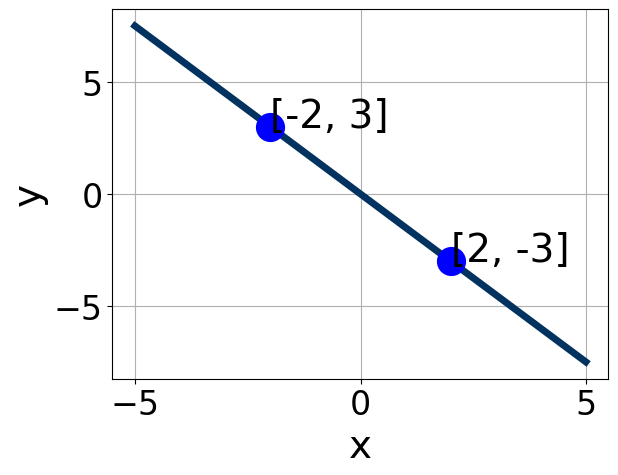
\includegraphics[width=0.5\textwidth]{../Figures/linearGraphToStandardC.png}
\end{center}
\begin{enumerate}[label=\Alph*.]
\item \( A \in [2.2, 4.6], \hspace{3mm} B \in [-2.63, -1.61], \text{ and } \hspace{3mm} C \in [-3, 2] \)
\item \( A \in [-0.3, 2.1], \hspace{3mm} B \in [0.88, 1.2], \text{ and } \hspace{3mm} C \in [-3, 2] \)
\item \( A \in [2.2, 4.6], \hspace{3mm} B \in [1.41, 2.5], \text{ and } \hspace{3mm} C \in [-3, 2] \)
\item \( A \in [-0.3, 2.1], \hspace{3mm} B \in [-1.02, -0.99], \text{ and } \hspace{3mm} C \in [-3, 2] \)
\item \( A \in [-3.9, -0.7], \hspace{3mm} B \in [-2.63, -1.61], \text{ and } \hspace{3mm} C \in [-3, 2] \)

\end{enumerate} }
\litem{
Write the equation of the line in the graph below in Standard form $Ax+By=C$. Then, choose the intervals that contain $A, B, \text{ and } C$.
\begin{center}
    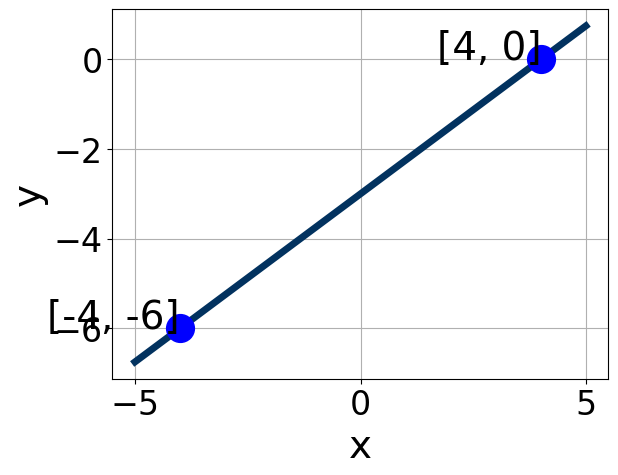
\includegraphics[width=0.5\textwidth]{../Figures/linearGraphToStandardCopyC.png}
\end{center}
\begin{enumerate}[label=\Alph*.]
\item \( A \in [1.9, 3.7], \hspace{3mm} B \in [3.6, 5], \text{ and } \hspace{3mm} C \in [-22, -15] \)
\item \( A \in [0.4, 2.7], \hspace{3mm} B \in [-1.3, -0.5], \text{ and } \hspace{3mm} C \in [4, 11] \)
\item \( A \in [0.4, 2.7], \hspace{3mm} B \in [0.5, 2], \text{ and } \hspace{3mm} C \in [-11, 1] \)
\item \( A \in [1.9, 3.7], \hspace{3mm} B \in [-4.3, -3.5], \text{ and } \hspace{3mm} C \in [19, 24] \)
\item \( A \in [-5.8, -0.2], \hspace{3mm} B \in [-4.3, -3.5], \text{ and } \hspace{3mm} C \in [19, 24] \)

\end{enumerate} }
\litem{
Find the equation of the line described below. Write the linear equation as $ y=mx+b $ and choose the intervals that contain $m$ and $b$.\[ \text{Parallel to } 8 x - 9 y = 4 \text{ and passing through the point } (-8, -6). \]\begin{enumerate}[label=\Alph*.]
\item \( m \in [1.06, 1.28] \hspace*{3mm} b \in [-0.2, 1.2] \)
\item \( m \in [0.35, 1.1] \hspace*{3mm} b \in [-2.9, -0.2] \)
\item \( m \in [0.35, 1.1] \hspace*{3mm} b \in [-0.2, 1.2] \)
\item \( m \in [0.35, 1.1] \hspace*{3mm} b \in [1.7, 2.5] \)
\item \( m \in [-1.02, 0.67] \hspace*{3mm} b \in [-14.3, -11.8] \)

\end{enumerate} }
\litem{
First, find the equation of the line containing the two points below. Then, write the equation as $ y=mx+b $ and choose the intervals that contain $m$ and $b$.\[ (-10, -6) \text{ and } (11, -11) \]\begin{enumerate}[label=\Alph*.]
\item \( m \in [-0.28, -0.15] \hspace*{3mm} b \in [-12.38, -5.38] \)
\item \( m \in [-0.28, -0.15] \hspace*{3mm} b \in [-22, -14] \)
\item \( m \in [-0.28, -0.15] \hspace*{3mm} b \in [0, 5] \)
\item \( m \in [-0.28, -0.15] \hspace*{3mm} b \in [5.38, 10.38] \)
\item \( m \in [0.04, 0.53] \hspace*{3mm} b \in [-14.62, -11.62] \)

\end{enumerate} }
\litem{
Solve the equation below. Then, choose the interval that contains the solution.\[ -17(-9x -7) = -8(10x -14) \]\begin{enumerate}[label=\Alph*.]
\item \( x \in [0.48, 1.32] \)
\item \( x \in [-1.05, -0.62] \)
\item \( x \in [-0.19, 0.24] \)
\item \( x \in [-3.76, -1.74] \)
\item \( \text{There are no real solutions.} \)

\end{enumerate} }
\litem{
Find the equation of the line described below. Write the linear equation as $ y=mx+b $ and choose the intervals that contain $m$ and $b$.\[ \text{Parallel to } 9 x + 5 y = 10 \text{ and passing through the point } (4, -10). \]\begin{enumerate}[label=\Alph*.]
\item \( m \in [-3.7, -1.1] \hspace*{3mm} b \in [2.8, 4.8] \)
\item \( m \in [-3.7, -1.1] \hspace*{3mm} b \in [-14, -11] \)
\item \( m \in [1.2, 3.1] \hspace*{3mm} b \in [-19.2, -16.2] \)
\item \( m \in [-3.7, -1.1] \hspace*{3mm} b \in [-6.8, -0.8] \)
\item \( m \in [-1.5, 0.3] \hspace*{3mm} b \in [-6.8, -0.8] \)

\end{enumerate} }
\litem{
Solve the equation below. Then, choose the interval that contains the solution.\[ -4(18x -3) = -6(-9x + 2) \]\begin{enumerate}[label=\Alph*.]
\item \( x \in [-0.17, 0.06] \)
\item \( x \in [-0.17, 0.06] \)
\item \( x \in [0.12, 0.54] \)
\item \( x \in [-0.17, 0.06] \)
\item \( \text{There are no real solutions.} \)

\end{enumerate} }
\litem{
Solve the linear equation below. Then, choose the interval that contains the solution.\[ \frac{4x + 7}{3} - \frac{8x + 5}{6} = \frac{6x -9}{7} \]\begin{enumerate}[label=\Alph*.]
\item \( x \in [4.1, 6.5] \)
\item \( x \in [2.8, 4.3] \)
\item \( x \in [12.6, 15] \)
\item \( x \in [-1, 2.8] \)
\item \( \text{There are no real solutions.} \)

\end{enumerate} }
\litem{
First, find the equation of the line containing the two points below. Then, write the equation as $ y=mx+b $ and choose the intervals that contain $m$ and $b$.\[ (9, -4) \text{ and } (-2, -8) \]\begin{enumerate}[label=\Alph*.]
\item \( m \in [0, 0.65] \hspace*{3mm} b \in [-13.21, -12.67] \)
\item \( m \in [0, 0.65] \hspace*{3mm} b \in [6.64, 9.55] \)
\item \( m \in [0, 0.65] \hspace*{3mm} b \in [-7.46, -6.96] \)
\item \( m \in [-0.93, 0.29] \hspace*{3mm} b \in [-10.03, -7.79] \)
\item \( m \in [0, 0.65] \hspace*{3mm} b \in [-6.97, -4.84] \)

\end{enumerate} }
\litem{
Solve the linear equation below. Then, choose the interval that contains the solution.\[ \frac{6x -4}{7} - \frac{4x -6}{5} = \frac{-3x -4}{4} \]\begin{enumerate}[label=\Alph*.]
\item \( x \in [-0.3, 1.2] \)
\item \( x \in [-3, -1.8] \)
\item \( x \in [-1.1, -0.1] \)
\item \( x \in [-9, -6.9] \)
\item \( \text{There are no real solutions.} \)

\end{enumerate} }
\end{enumerate}

\end{document}